% ..............................................................................
% Demo of the fau-beamer template.
%
% Copyright 2022 by Tim Roith <tim.roith@fau.de>
%
% This program can be redistributed and/or modified under the terms
% of the GNU Public License, version 2.
%
% ------------------------------------------------------------------------------

% ------------------------------------------------------------------------------
\section{Topic Orientation}
% ..............................................................................
% Review
\subsection{Seminar Review}
\begin{frame}[t]{Seminar Review}{What did we learn in this seminar?}
	\begin{itemize}
		
		\item \textbf{Significance testing (Statistical methods)}
		\begin{itemize}
			\item Null hypothesis, p-value, chi-square test
		\end{itemize}
		\bigbreak
			
		\item \textbf{Corpus design}
		\begin{itemize}
			\item Social media corpora
			\item Spoken language corpora
		\end{itemize}
		\bigbreak
		
		\item \textbf{Application of  Corpus Linguistics (Results Interpretation)}
		\begin{itemize}
			\item Critical discourse analysis
			\item Translation studies
			\item Pragmatic studies
		\end{itemize}
		
	\end{itemize}
\end{frame}


% ..............................................................................
% Procedures
\subsection{Procedures of a Corpus Linguistics research}
\begin{frame}{Procedures of a Corpus Linguistics research}
	\begin{figure}
		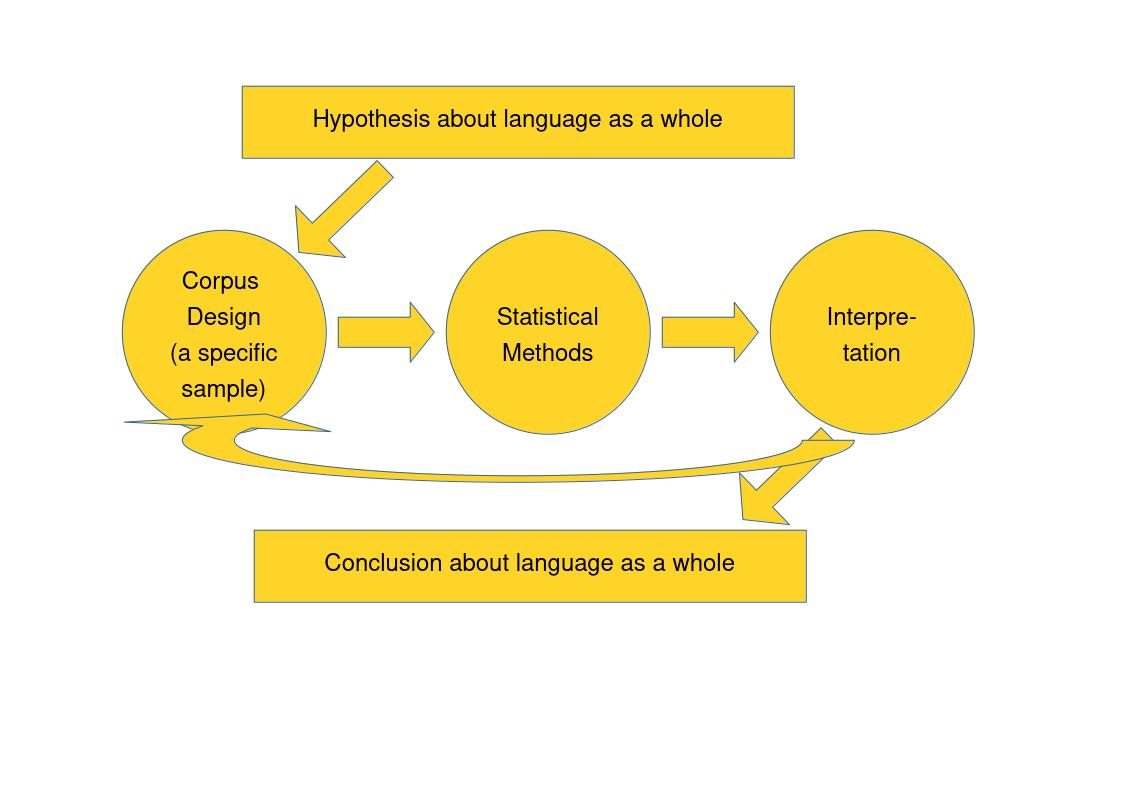
\includegraphics[width=.7\textwidth]{Figures/Procedures.jpg}
		\caption{Three steps in a typical CL research}
	\end{figure}
\end{frame}


% ..............................................................................
%Topic  key word
\subsection{Topic key word}
\begin{frame}[t]{Topic key word}{Evert: Reflection of Statistical Methods in Corpus Linguistics}
	
	\begin{itemize}
		\item \textit{why should we apply statistical methods (based on the \textbf{random sample} model) at all?} (in corpus linguistics)
		\begin{itemize}
			\item Evert, Stefan. "How Random is a Corpus? The Library Metaphor" Zeitschrift für Anglistik und Amerikanistik, vol. 54, no. 2, 2006, pp. 177-190.
		\end{itemize}
		\bigbreak
		\item What does \textbf{Randomness} actually mean in Corpus Linguistics?
		\bigbreak
		
		\item Sources of \textbf{(non-)Randomness}: Corpus design
		\bigbreak
		
		\item Validating the \textbf{(non-)Randomness}: Results interpretation 
	\end{itemize}
	
\end{frame}

